\documentclass[11pt,a4paper]{article}

\usepackage[margin=1.1in]{geometry}
\usepackage{amsmath,amssymb,amsthm,mathtools}
\usepackage[T1]{fontenc}
\usepackage{microtype}
\microtypesetup{expansion=false}
\usepackage{tikz}
\usetikzlibrary{positioning,arrows.meta,calc,fit,backgrounds,patterns}
\usepackage{booktabs}
\usepackage{listings}
\usepackage{stmaryrd}
\usepackage[hidelinks]{hyperref}
\usepackage{enumitem}

\theoremstyle{plain}
\newtheorem{theorem}{Theorem}
\newtheorem{proposition}[theorem]{Proposition}
\newtheorem{lemma}[theorem]{Lemma}
\newtheorem{corollary}[theorem]{Corollary}
\newtheorem{conjecture}[theorem]{Conjecture}
\theoremstyle{definition}
\newtheorem{definition}[theorem]{Definition}
\newtheorem{observation}[theorem]{Observation}
\newtheorem{example}[theorem]{Example}
\theoremstyle{remark}
\newtheorem{remark}[theorem]{Remark}

\newcommand{\rhoc}{\textsf{rho}}
\newcommand{\Nil}{\mathbf{0}}
\newcommand{\sepc}{\mathbin{\big|}}
\newcommand{\Hq}{\mathsf{H}}
\newcommand{\out}{\mathsf{out}}
\newcommand{\inn}{\mathsf{in}}
\newcommand{\Rnn}{\mathbb{R}_{\geq 0}}
\newcommand{\Cx}{\mathbb{C}}
\newcommand{\Terms}{\mathcal{T}}
\newcommand{\Cfg}{\mathcal{C}}
\newcommand{\Wt}{\mathcal{W}}
\newcommand{\Red}{\mathrm{Red}}
\newcommand{\prop}{\mathbf{a}}
\newcommand{\wmap}{w}
\newcommand{\dpt}{d}
\newcommand{\gfac}{g}
\newcommand{\funds}{\mathrel{\vdash_{\!\$}}}
\newcommand{\class}{\mathrm{cls}}
\newcommand{\Lop}{L}
\newcommand{\Heff}{H_{\mathrm{eff}}}
\newcommand{\dbr}[1]{\llbracket #1 \rrbracket}

\lstdefinestyle{rho}{
  basicstyle=\ttfamily\footnotesize,
  keywordstyle=\bfseries,
  commentstyle=\itshape,
  morekeywords={new,in,for,contract,match,if,else,true,false,Nil,where,and,or,not,
                exists,forall,nu,rules,rewrites,equations,types,language,name},
  morecomment=[l]{//},
  columns=fullflexible,
  breaklines=true,
  breakatwhitespace=false,
  showstringspaces=false,
  frame=none,
  xleftmargin=1em
}
\lstset{style=rho}

\title{\textbf{Weighted Graph-Structured Lambda Theories}\\[0.4em]
\large Stochastic and quantum execution for MeTTaIL, with recurrent\\
neural networks as a worked example}
\author{A F1R3FLY.io working note}
\date{August 2026}

\begin{document}
\maketitle

\begin{abstract}
We equip the rewrite rules of a finitely presentable graph-structured lambda theory (GSLT), as
presented in MeTTaIL, with \emph{weight maps}: finite maps whose keys are spatial--behavioural
formulae refining the left-hand side of a rule and whose values are weights. A weight map instance
is part of a state specification, so a rewrite may update it; weights are therefore dynamic. We
develop the construction in three movements. First, we impose a \emph{partition discipline} on the
key set --- the refinements of a rule's left-hand side must be pairwise exclusive and jointly
exhaustive --- and show that this single requirement is what makes the weighting a total,
single-valued classification of redexes, forces the generated logic's target specification to be
Boolean, and, in the complex-valued case, makes the refinement classes a projective measurement.
Second, with weights in $\Rnn$ we define propensity as
$\prop = \wmap(\varphi)\cdot\sum_k \gfac(k)$ over classified, funded redex positions and obtain a
Gillespie simulator; we prove that the construction restricted to the $\pi$-calculus, static maps,
and channel-identity keys is exactly the Stochastic Pi Machine, and that dynamic maps take it
strictly beyond. Third, with weights in $\Cx$ we read each refinement entry as a Lindblad jump
operator, obtain a quantum continuous-time Markov chain in the sense of Xu, Mei, Guan and Yu, and
show that the Gillespie algorithm is the quantum-jump unravelling at zero Hamiltonian --- which is
the precise sense in which the quantum simulator is \emph{Gillespie-inspired}. The worked example is
a recurrent neural network in a weighted \rhoc\ theory: neurons are persistent for-comprehensions,
synaptic efficacies live in the weight map rather than in the payload, thresholds are join
structure, the logistic response is emergent from the chain rather than written into a term, and
Hebbian plasticity is exactly the refinement entries' update functions --- so that learning and
inference are the same transition relation, differing only in which component of the state they
touch.
\end{abstract}

\tableofcontents

\section{Introduction}
\label{sec:intro}

A rewrite rule's left-hand side is a type. Terms inhabit it; the rule fires at its inhabitants. This
note is about what happens when one refines that type and attaches a number to each refinement.

The move is small to state and consequential to develop. A GSLT is a triple $(\Sigma, E, R)$: a
signature which is in general a lambda theory, a set of equations imposing a structural congruence,
and an adjoined graph of rewrite rules \cite{omnibus}. Given such a presentation, the OSLF family of
algorithms generates a logic from it, with one structural connective per term former of $\Sigma$ and
one context-labelled modality per rule of $R$ together with a choice of redex position
\cite{omnibus,classifier}. The formulae of that generated logic are exactly the vocabulary in which
one can refine a rule's left-hand side --- and they are generated, not designed, so the refinements
come for free with the theory. To weight a rule is to give a finite map
\[
\varphi_1 \mapsto v_1, \quad \ldots, \quad \varphi_m \mapsto v_m
\]
from such refinements to weights. A term's redexes are then classified by which refinement they
satisfy, and the weights turn the set of enabled redexes into a distribution.

Two things distinguish this from the existing literature on stochastic process calculi.

\paragraph{Keys are formulae, not names.} In Priami's stochastic $\pi$-calculus \cite{priami} and in
Phillips and Cardelli's Stochastic Pi Machine (SPiM) \cite{spim,spim-sim}, a rate is attached to a
\emph{channel}. That is one refinement among many: ``this redex is a communication on $n$'' is a
particular formula in the generated logic, and there is no reason the modeller should be restricted
to it. Once keys are formulae, a rate may depend on the shape of the payload, on the structure of
the surrounding term as seen through the separating conjunction, on the namespace the channel
belongs to, or on any Boolean combination of these. Channel identity is recovered as the degenerate
case (\S\ref{sec:spim}).

\paragraph{Maps are state, not declaration.} A weight map instance is part of a state
specification. A rule's refinement entries therefore carry not only a weight but an \emph{update
function} on the whole map, applied when the rule fires. Rates change during execution. SPiM does
not permit this --- its rates are fixed at declaration --- and the restriction is not incidental to
its design but constitutive of it, since a static rate function is what makes the underlying object
a time-homogeneous CTMC over terms alone. We recover Markovianity by a different route: the weight
map is \emph{in} the state, so the chain is over configurations $(P, \wmap)$ rather than over terms
(\S\ref{sec:gillespie}). This is the technical content of ``the map may be updated,'' and it is what
the worked example of \S\ref{sec:rnn} needs, because plasticity is nothing other than a weight-map
update.

Two further points of scope. The construction is generic over the GSLT: it applies to any theory
one can write down in MeTTaIL's \texttt{language!} block \cite{mettail}, so one obtains a stochastic
machine for the ambient calculus, for a user-defined DSL, or for the \rhoc\ calculus, by writing the
theory rather than by writing a simulator. And the weight codomain is a parameter. We treat two
instances: $\Rnn$, giving classical Gillespie simulation (\S\ref{sec:gillespie}); and $\Cx$, giving
a quantum continuous-time Markov chain in the sense of \cite{qctmc} and a Gillespie-inspired
trajectory simulation for it (\S\ref{sec:quantum}). A third instance --- weights in a quantale,
giving a fuzzy calculus --- is deliberately out of scope here; see \cite{fuzzy}.

\paragraph{What is new.} Beyond the two distinguishing points above:
\begin{enumerate}[label=(\roman*),leftmargin=2.2em]
\item The \emph{partition discipline} of \S\ref{sec:refinement}, and the observation that it is not
a technicality but the condition under which weighting is well defined at all --- with three
independent payoffs (totality of the classifier, a Boolean demand on the target logic
specification, and a projective measurement in the quantum case).
\item A propensity formula (\S\ref{sec:propensity}) that separates four factors which the literature
usually conflates: the refinement's weight, a geometric factor accumulated up the context rules,
redex multiplicity, and a funding gate supplied by cost accounting.
\item Theorem~\ref{thm:spim}: SPiM is the construction's restriction, exactly.
\item Theorem~\ref{thm:jump-gillespie}: the Gillespie algorithm is the quantum-jump unravelling at
zero Hamiltonian and diagonal jump structure --- so ``Gillespie-inspired'' is a theorem about
degeneration, not an analogy.
\item The observation (\S\ref{sec:qctmc-logic}) that the OSLF-generated formulae supply exactly the
atomic propositions that quantum CTMC model checking otherwise has to be handed by hand.
\item The recurrent-neural-network example of \S\ref{sec:rnn}, in which the synaptic weights live in
the weight map, the threshold lives in the join structure of a for-comprehension, the logistic
response is emergent, and learning is a weight-map update performed by the same rewrite that
performs inference.
\end{enumerate}

\paragraph{Where this note sits.} It supplies the construction that \cite{scientist} cites as
\emph{Stochastic simulation for decorated ciGSLTs} and fills the placeholder section of
\cite{mettacalc}. It depends on \cite{omnibus} for GSLTs and OSLF, on \cite{classifier} and
\cite{scientist} for the shape of the generated spatial--behavioural logic --- which is spelled out
in those papers and not yet present in the implementation branch --- and on \cite{costmonad} for
cost accounting, which enters only in \S\ref{sec:cost} and only as a gate.

\section{Background, compressed}
\label{sec:background}

We recall only what the construction uses, and forward everything else to \cite{omnibus}.

\subsection{GSLTs and their presentations}

A \emph{graph-structured lambda theory} is a triple $(\Sigma, E, R)$. The signature $\Sigma$ is a
lambda theory --- terms may contain variables, and binding is part of the presentation, which is
what distinguishes the setting from graph-enriched Lawvere theories. $E$ is a set of equations
imposing a structural congruence $\equiv$ on terms. $R$ is a graph of rewrite rules adjoined to the
structure as a Lawvere theory of graphs, with source and target maps satisfying the minimal
requisite equations. The adjective \emph{graph-structured} captures the rewrites; \emph{lambda
theory} captures term languages with variables.

Rules come in two kinds, and the distinction is load-bearing throughout this note.

\begin{definition}[Base and context rules]
\label{def:rules}
A \emph{base rule} is hypothesis-free:
\[
r \,.\; \vdash\; L \;\leadsto\; R,
\]
with $L, R$ terms of some sort $\tau$ over $\Sigma$, possibly with pattern variables. A
\emph{context rule} is conditional on a rewrite:
\[
c \,.\; \mid S \leadsto T \;\vdash\; C[S] \;\leadsto\; C[T],
\]
for a one-hole context former $C$. Base rules are the ground of the dynamics; context rules are
\emph{addressing} --- they say where a base rule may fire, not that anything happens.
\end{definition}

This is MeTTaIL's actual surface syntax for its \texttt{rewrites} block \cite{mettail}. In the
\rhoc\ presentation, \texttt{Exec} and the communication rule are base; \texttt{ParCong} and
\texttt{NewCong} are context rules.

An \emph{interactive} GSLT is one whose base rules' left-hand sides are headed by a distinguished
family of formers $K$ --- the interaction cut --- across which program and environment meet:
application for the lambda calculus, parallel composition for CCS, $\pi$ and \rhoc. A
\emph{continued} interactive GSLT (ciGSLT) additionally has surfaces and continuations. Everything
below is stated for ciGSLTs, though only the interactive structure is used.

\subsection{Locations}

Write $\partial \Terms$ for the space of one-hole contexts, in the McBride-derivative sense: a
location is a pair $(\partial T, T)$ of a context and the term type. We use $\partial \Terms$ as a
single object playing three roles, as in \cite{omnibus}: the index set of the generated modalities,
the labels on the transition system, and the positions inside a term. It is this identification that
lets a weight be attached to a \emph{position} and read as a modality.

\begin{definition}[Redex]
\label{def:redex}
Let $r \,.\; \vdash L \leadsto R$ be a base rule and $P$ a term. A \emph{redex of $r$ in $P$} is a
\emph{selection} of a one-hole context $k \in \partial\Terms$ and a substitution $\sigma$ for the
pattern variables of $L$ from the decomposition of $P$, such that $P \equiv k[L\sigma]$. Two redexes
are identified when they select the same occurrences; interchanging two occurrences of
$\equiv$-equal subterms yields \emph{distinct} redexes, which happen to have $\equiv$-equal
contracta. Write $\Red_r(P)$ for the set of redexes of $r$ in $P$, and
$\Red(P) = \coprod_r \Red_r(P)$.
\end{definition}

$\Red_r(P)$ is finite for finite $P$ and finitely many rules. The convention on identification is
Gillespie's, and it is the one that matters: two molecules of the same species offer two ways for a
reaction to occur, not one, and a stochastic simulator that identifies them runs at half speed. In
an associative--commutative setting the reactants are drawn from a multiset, so $|\Red_r(P)|$ is a
count of selections from a bag --- $\mathrm{In}\cdot\mathrm{Out}$ for a binary interaction drawing
one reactant from each of two species, $\binom{n}{2}$ for one drawing two from the same species.
Structural congruence is used to \emph{find} the decompositions, not to collapse them.
Remark~\ref{rem:distinct-contracta} records what happens when distinct redexes do share a contractum.

\subsection{The generated logic}
\label{sec:logic}

The following is generated by OSLF from the presentation and is not ours to design. We state it for
the \rhoc\ calculus --- term formers $\Nil$, $*n$, $n!(Q)$, $\texttt{for}(x \leftarrow n)P$,
parallel composition, and $@P$, with parallel composition associative--commutative and a single
communication rewrite --- and note that everything transfers verbatim to any other presentation,
with the connective list changing to match the formers. The presentation follows
\cite[\S2]{classifier} and \cite[\S3]{scientist}; it is not present in the implementation branch,
whose logic is still under development.

\paragraph{Structural connectives.} One connective per term former. $\out(n)\varphi$ holds of
$n!(Q)$ with $Q \models \varphi$; $\inn(n)\varphi$ is the analogue on receipts. Because parallel
composition is associative--commutative, the generated connective for it is a separating
conjunction:
\[
P \models \varphi \sepc \psi
\iff
P \equiv Q \sepc R \text{ with } Q \models \varphi,\ R \models \psi .
\]

\paragraph{Behavioural modalities.} One primitive modality $\langle K_j \rangle$ per rewrite rule
\emph{and choice of redex position}, labelled by the one-hole context in which the step fires. The
index is not decoration. For \rhoc, with a single interaction rule, all the information in a label
is in the position: for $P \equiv K_j[\,\texttt{for}(x \leftarrow n)Q \sepc n!(Q')\,]$ the label
$K_j$ is everything else. Thus $\exists j.\,\langle K_j\rangle\varphi$ and
$\forall j.\,[K_j]\varphi$ quantify over redex positions, and a bare $\langle K \rangle$ abbreviates
the existential.

\paragraph{Name predicates.} A name is a quoted process, so
\[
n \models @\varphi \iff n = @P \text{ with } P \models \varphi ,
\]
which is namespace logic \cite{namespace}: a namespace is described by a property rather than
enumerated. This matters in \S\ref{sec:rnn}, where synapses are picked out by structured names.

\paragraph{Propositional layer.} Conjunction and $\top$ come from the finite-limits fragment;
disjunction, implication and negation require more, and a target specification supplies them or does
not \cite{omnibus}. \S\ref{sec:boolean} shows that weighting \emph{forces} the choice.

\paragraph{Additions.} A greatest fixed point $\nu X.\varphi$ with $X$ positive; the hidden-name
quantifier $\Hq x.\varphi$; graded separation $\varphi \sepc_k \psi$ \cite[\S2.3]{classifier}. We
use $\nu$ only in \S\ref{sec:rnn-uniform}.

\begin{definition}[Depth]
\label{def:depth}
The depth $\dpt(\varphi)$ of a structural formula is the maximal nesting of term-former connectives
and prefixes: $\dpt(\top) = 0$, $\dpt(\out(n)\varphi) = \dpt(\inn(n)\varphi) = 1 + \dpt(\varphi)$,
$\dpt(\varphi \sepc \psi) = \max(\dpt(\varphi), \dpt(\psi))$, $\dpt(@\varphi) = \dpt(\varphi)$,
$\dpt(\Hq x.\varphi) = 1 + \dpt(\varphi)$.
\end{definition}

\subsection{Ideal logic, checkable fragment}

One methodological commitment governs \S\ref{sec:refinement}. Following \cite[\S1.3]{classifier}, we
distinguish the \emph{ideal} logic, adequate for the idealised calculus and the thing that
\emph{defines} a semantic notion, from \emph{fragments}, restricted so that model checking
terminates, which \emph{decide} it. A logic whose model checking terminates is necessarily not
adequate for the whole of a Turing-complete host. The relevance here is sharp and appears at
Requirement~\ref{req:dec}: a simulator evaluates its key formulae at every step, so keys must come
from a checkable fragment. What is elsewhere a methodological trade-off is here an executability
constraint.

\section{Refining a left-hand side}
\label{sec:refinement}

\subsection{The keys}

Fix a base rule $r \,.\; \vdash L \leadsto R$ with $L$ of sort $\tau$. The set of redexes of $r$ is
carved out by the shape of $L$; we want to subdivide it. Write $L^\sharp$ for the structural formula
that characterises the left-hand side pattern --- for the \rhoc\ communication rule,
$L^\sharp = \inn(n)\top \sepc \out(n)\top$ with $n$ existentially bound. The candidate keys are the
formulae of the generated logic that \emph{refine} $L^\sharp$.

\begin{definition}[Refinement]
\label{def:refinement}
A formula $\varphi$ \emph{refines} $L^\sharp$, written $\varphi \sqsubseteq L^\sharp$, when
$\models \varphi \Rightarrow L^\sharp$. The refinements of $L^\sharp$, ordered by entailment, form
the \emph{refinement lattice} $\mathcal{R}(r)$ of the rule.
\end{definition}

We now impose three requirements on a key set $\Phi_r \subseteq \mathcal{R}(r)$. The first is the
substantial one.

\begin{definition}[Partition discipline]
\label{def:partition}
$\Phi_r = \{\varphi_1, \ldots, \varphi_m\}$ is a \emph{partition of $r$} when
\begin{enumerate}[label=(P\arabic*),leftmargin=3em]
\item \emph{Exclusivity}: $\models \neg(\varphi_i \wedge \varphi_j)$ for all $i \neq j$;
\item \emph{Exhaustiveness}: $\models L^\sharp \Rightarrow \bigvee_{i} \varphi_i$.
\end{enumerate}
\end{definition}

\begin{definition}[Requirements on a key set]
\label{def:reqs}
A key set is \emph{admissible} when it is a partition and, in addition:
\begin{enumerate}[label=(R\arabic*),leftmargin=3em]
\item\label{req:dec} \emph{Decidability}: each $\varphi_i$ lies in a fragment for which model
checking terminates on the terms of interest.
\item\label{req:loc} \emph{Locality}: $\dpt(\varphi_i) \le \alpha_r < \infty$ for all $i$, for some
bound $\alpha_r$ fixed with the rule.
\end{enumerate}
\end{definition}

\ref{req:dec} is forced by execution: a simulator must classify every enabled redex before it can
sample, so a key whose evaluation may diverge is a key that stops the simulation. \ref{req:loc} is
forced by \emph{efficient} execution, and pays off in Lemma~\ref{lem:locality}.

\subsection{What the partition buys}

\begin{proposition}[Classification]
\label{prop:classify}
Let $\Phi_r$ be a partition of $r$. Then the assignment
\[
\class_r : \Red_r(P) \longrightarrow \Phi_r,
\qquad
\class_r(k, \sigma) = \text{the unique } \varphi_i \text{ with } L\sigma \models \varphi_i
\]
is a total function, for every term $P$.
\end{proposition}

\begin{proof}
$(k,\sigma) \in \Red_r(P)$ gives $P \equiv k[L\sigma]$, so $L\sigma \models L^\sharp$ by
construction of $L^\sharp$. Exhaustiveness gives $L\sigma \models \varphi_i$ for some $i$, which is
totality; exclusivity gives at most one such $i$, which is single-valuedness. Well-definedness on
$\equiv$-classes holds because satisfaction is $\equiv$-invariant, the generated connectives being
generated from $\Sigma$ modulo $E$.
\end{proof}

This is exactly what fails without the discipline, and it fails in two directions. Without
exhaustiveness the weighting is partial: some enabled redexes have no rate, and one must invent a
convention (fire them at rate zero? at a default rate? refuse to run?) that is not part of the
specification. Without exclusivity the weighting is multi-valued, and one must invent an
\emph{aggregation} (take the most specific key, if a unique minimum exists; sum the weights of all
satisfied keys; take the maximum). Each convention is defensible and each yields a different
simulator from the same specification, which is precisely the situation a specification exists to
prevent.

\begin{remark}[Completing a partition is cheap]
\label{rem:default}
The discipline is less onerous than it looks. Given any pairwise-exclusive family
$\{\varphi_1,\dots,\varphi_m\}$, the family
$\{\varphi_1,\dots,\varphi_m,\ \varphi_\bot\}$ with
$\varphi_\bot := L^\sharp \wedge \neg\bigvee_i \varphi_i$ is a partition, and a modeller who wants
the unlisted redexes inert simply sets $\wmap(\varphi_\bot) = 0$. Exclusivity is the real
constraint; exhaustiveness is a completion. In practice, keys of the form ``the redex is a
communication on channel $n$,'' indexed by distinct $n$, are exclusive for free.
\end{remark}

\subsection{The partition forces a Boolean target specification}
\label{sec:boolean}

\begin{proposition}[Boolean demand]
\label{prop:boolean}
Stating the partition discipline requires negation, conjunction and disjunction in the generated
logic. Consequently a weighted GSLT cannot be specified over a target logic specification carrying
only the finite-limits fragment.
\end{proposition}

\begin{proof}
Immediate from (P1) and (P2): (P1) mentions $\neg$ and $\wedge$, (P2) mentions $\Rightarrow$ and
$\bigvee$. Finite limits supply $\wedge$ and $\top$ only \cite{omnibus}.
\end{proof}

This is worth pausing on, because it is a convergence rather than an inconvenience. The omnibus
identifies possession of something like a negation and a conjunction as exactly the condition under
which a generated logic enjoys an adequacy theorem, and notes that Hypercube-style members of the
OSLF family, which generate type systems, offer no such thing \cite{omnibus}. Proposition
\ref{prop:boolean} says that the weighting apparatus makes the same demand for an independent
reason. The moral: \emph{one cannot weight a theory whose generated logic is too weak to be
adequate for it.} A weighting is a claim about which behaviours are distinguishable enough to be
priced differently, and that claim needs the same expressive power as the claim that they are
distinguishable at all.

Requirement \ref{req:dec} then pulls the other way, since a terminating fragment is necessarily
inadequate for a Turing-complete host. The two are not in conflict, because they apply to different
artifacts: adequacy is a property of the ideal logic in which the specification is \emph{stated},
and termination is a property of the fragment in which the keys are \emph{evaluated}. A modeller
writes a partition in the ideal logic, then checks that the particular keys chosen happen to lie in
a checkable fragment. \S\ref{sec:rnn} exhibits keys of depth $2$, for which the check is trivial.

\subsection{Locality}

\begin{lemma}[Locality of reclassification]
\label{lem:locality}
Let all keys of all rules have depth at most $\alpha$, let $P \equiv k[L\sigma]$ and let
$P' \equiv k[R\sigma]$ be the result of firing that redex. Then for any redex $(k', \sigma')$ of any
rule surviving in $P'$ whose position is at distance greater than $\alpha + |L| + |R|$ from the fired
position in the term tree, $\class(k',\sigma')$ is unchanged.
\end{lemma}

\begin{proof}
A formula of depth $\alpha$ evaluated at a position inspects only the subterm within $\alpha$ nested
formers of that position, and the separating conjunction inspects a decomposition of that subterm,
not of the whole. The rewrite replaces $L\sigma$ by $R\sigma$ and leaves $k$ pointwise fixed, so any
window of radius $\alpha$ disjoint from the replaced material sees an identical subterm. The offset
$|L| + |R|$ accounts for windows that overlap the replaced region.
\end{proof}

The point is algorithmic. Recomputing $\class$ over the whole term at every step makes the simulator
quadratic in term size; Lemma~\ref{lem:locality} licenses an incremental propensity update in the
style of Gibson and Bruck's next-reaction method \cite{gibson-bruck}, touching only a bounded
neighbourhood of the fired redex. This is where \ref{req:loc} earns its place, and it is also the
reason to prefer shallow keys where the modelling permits.

\section{Weighted rewrite systems}
\label{sec:weighted}

\subsection{The weight codomain}

Weights are drawn from a commutative semiring $\mathcal{K}$. We treat two instances:
\[
\mathcal{K} = \Rnn = (\Rnn, +, \cdot, 0, 1)
\qquad\text{and}\qquad
\mathcal{K} = \Cx .
\]

\begin{remark}[Rates, not probabilities]
\label{rem:rnn}
We take the real codomain to be $\Rnn$ rather than the unit interval. A Gillespie waiting time is
$\tau = a_0^{-1}\ln(1/u)$ and therefore carries units of time; a weight is a rate, with units of
inverse time, and there is nothing to normalise it against. The unit interval is available as a
derived presentation: fixing a global clock rate $\lambda \geq a_0$ and setting
$p_i = a_i / \lambda$ gives the uniformised discrete-time chain, whose jump probabilities do live in
$[0,1]$ and whose sojourn is a fixed exponential of rate $\lambda$. Uniformisation is a good
implementation strategy and a bad specification, because $\lambda$ must dominate the propensity of
every reachable configuration and the dynamic weight maps of \S\ref{sec:dynamic} make that bound a
global proof obligation rather than a local one. We specify in $\Rnn$ and let an implementation
uniformise if it wishes.
\end{remark}

For $\Cx$ we do require $|z| \le 1$ on each entry, for the reason given at
Definition~\ref{def:jump}: an entry becomes a jump operator, and the resulting semigroup must be
trace non-increasing.

\subsection{Weight maps and augmented rules}

\begin{definition}[Weight map]
\label{def:wmap}
Let $(\Sigma, E, R)$ be a GSLT with admissible key sets $\Phi_r$ for each base rule $r$. A
\emph{weight map} is a function
\[
\wmap : \textstyle\coprod_{r} \Phi_r \longrightarrow \mathcal{K}.
\]
Write $\Wt$ for the set of weight maps. Since each $\Phi_r$ is finite and there are finitely many
rules, $\Wt \cong \mathcal{K}^N$ for a fixed $N$.
\end{definition}

\begin{definition}[Configuration]
\label{def:config}
A \emph{configuration} is a pair $\mathfrak{c} = (P, \wmap)$ with $P$ a term modulo $\equiv$ and
$\wmap \in \Wt$. Write $\Cfg$ for the set of configurations.
\end{definition}

The phrase ``a map instance is part of a state specification'' is Definition~\ref{def:config}, and
everything downstream turns on it.

\begin{definition}[Augmented rules]
\label{def:augmented}
An \emph{augmented base rule} is
\[
r \,.\; \vdash\; L \leadsto R \;\; [\,\wmap_r\,]
\;\{\; \varphi_1 \Rightarrow (v_1, u_1), \;\ldots,\; \varphi_m \Rightarrow (v_m, u_m) \;\}
\]
where $\{\varphi_i\}$ is an admissible key set for $r$, $v_i \in \mathcal{K}$ are the initial
weights, and $u_i : \Wt \to \Wt$ are \emph{update functions} on the whole map. An \emph{augmented
context rule} is
\[
c \,.\; \mid S \leadsto T \;\vdash\; C[S] \leadsto C[T] \;\; [\,\gfac_c\,] \;\{\; f_c \;\}
\]
with $\gfac_c \in \Rnn$ a \emph{geometric factor} and $f_c : \Wt^* \times \Wt \to \Wt$ a
\emph{fold function}.
\end{definition}

The initial weight map is $\wmap_0(\varphi_i) = v_i$; the leading $[\wmap_r]$ is a per-rule scalar,
convenient in practice and formally absorbable into the $v_i$, which is how we treat it below.

\subsection{Why context rules carry a factor and not a propensity}
\label{sec:geometric}

The design decision that most distinguishes Definition~\ref{def:augmented} from the obvious
alternative is that context rules do not have propensities of their own.

The obvious alternative gives every rule, base and context alike, a weight and lets the simulator
select among all of them. It double-counts. A step of the transition system is a base rule firing
\emph{somewhere}; the context rules composing the path from the root to that somewhere are the
address of the firing, not additional events. In the vocabulary of the energetics reading of
OSLF-decorated GSLTs, structural rules are addressing, not dynamics, and incur no primitive cost.
Selecting a context rule and then a base rule as though they were independent draws makes a single
event into two.

So context rules contribute multiplicatively, to the propensity of the base firing they address:

\begin{definition}[Geometric factor]
\label{def:gfac}
Let $k \in \partial\Terms$ be a position, obtained by composing context rules $c_1, \ldots, c_p$
from the root inwards. Its \emph{geometric factor} is
$\gfac(k) = \prod_{q=1}^{p} \gfac_{c_q} \in \Rnn$.
\end{definition}

Setting every $\gfac_c = 1$ recovers ``addressing is free'' exactly, and is the default we recommend.
The reason to permit $\gfac_c \neq 1$ is that it is the natural home for a \emph{spatial} bias:
$\gfac$ is a weighting on the reduction graph's edges that depends only on where in the term the
interaction surfaces are, as against $\wmap(\varphi)$, which depends on what is being transferred.
This is the geometric-versus-matter split of the gravitation correspondence \cite{costspacetime}
appearing here as an implementation detail, and we flag it as such without pursuing it.

\subsection{Dynamics}
\label{sec:dynamic}

\begin{definition}[Weighted transition]
\label{def:transition}
Let $\mathfrak{c} = (P, \wmap)$ and let $(k,\sigma) \in \Red_r(P)$ with
$\class_r(k,\sigma) = \varphi_i$, the position $k$ composed of context rules $c_1, \ldots, c_p$.
Then $\mathfrak{c}$ steps to $\mathfrak{c}' = (P', \wmap')$ where
\[
P' \equiv k[R\sigma],
\qquad
\wmap' = f_{c_1}\!\big(\vec{\omega}_1,\; f_{c_2}(\vec{\omega}_2, \;\cdots\; f_{c_p}(\vec{\omega}_p,\; u_i(\wmap))\cdots)\big),
\]
the fold functions being applied from the redex outwards, with $\vec{\omega}_q$ the maps arising
from the sibling subterms at level $q$.
\end{definition}

In the common case where every $f_c$ is the projection onto its second argument --- ``the context
does not modify the map'' --- this collapses to $\wmap' = u_i(\wmap)$, and we write it so below.

\begin{definition}[The coalgebra]
\label{def:coalgebra}
Let $\mathcal{K}^{(-)}$ denote the free-$\mathcal{K}$-semimodule monad, $\mathcal{K}^{(X)}$ being
finitely supported functions $X \to \mathcal{K}$. A weighted GSLT determines a coalgebra
\[
\gamma : \Cfg \longrightarrow \mathcal{K}^{(\Cfg)},
\qquad
\gamma(\mathfrak{c})(\mathfrak{c}') \;=\; \sum_{\substack{(r,k,\sigma) \\ \text{stepping } \mathfrak{c} \to \mathfrak{c}'}} \wmap(\class_r(k,\sigma)) \cdot \gfac(k).
\]
\end{definition}

This is the target of the whole construction: a decorated ciGSLT plus an adequate
spatial--behavioural logic plus a weight-map decoration gives a $\mathcal{K}$-weighted coalgebra.
Assembling the decorations of a fixed theory into a category and taking the Grothendieck
construction gives the fibred form; the simulator is a functor out of it. We do not need the fibred
statement below and record it only to fix the picture.

\begin{remark}[Sum over derivations, not over targets]
The sum in Definition~\ref{def:coalgebra} runs over \emph{derivations} that reach $\mathfrak{c}'$,
not merely over the target. In $\Rnn$ this is the familiar statement that parallel routes to the
same state add their rates. In $\Cx$ it is the interference condition, and it is the reason the
quantum case is not a routine relabelling; see \S\ref{sec:interference}.
\end{remark}

\section{Propensity}
\label{sec:propensity}

The propensity of a rule at a refinement is where the construction is most easily got wrong, because
four independent factors are involved and the literature usually presents some of them fused. We
separate them.

\begin{definition}[Propensity]
\label{def:propensity}
Let $\mathfrak{c} = (P, \wmap)$ be a configuration, $r$ a base rule and $\varphi \in \Phi_r$. Put
\[
K(r, \varphi, P) \;=\; \{\, (k,\sigma) \in \Red_r(P) \;:\; \class_r(k,\sigma) = \varphi \,\}.
\]
The \emph{propensity} of $(r,\varphi)$ at $\mathfrak{c}$ is
\[
\prop(r,\varphi,\mathfrak{c})
\;=\;
\wmap(\varphi) \cdot \!\!\sum_{(k,\sigma) \in K(r,\varphi,P)}\!\! \gfac(k)\cdot \chi(r,k,\sigma),
\]
where $\chi \in \{0,1\}$ is the funding gate of \S\ref{sec:cost}, identically $1$ in the absence of
cost accounting. The \emph{total propensity} is
$\prop_0(\mathfrak{c}) = \sum_{r}\sum_{\varphi \in \Phi_r} \prop(r,\varphi,\mathfrak{c})$.
\end{definition}

The four factors:
\begin{description}[leftmargin=1.6em,style=nextline]
\item[$\wmap(\varphi)$ --- the rate constant.] What kind of interaction this is, priced. Dynamic:
this is the component update functions rewrite.
\item[$\gfac(k)$ --- the geometric factor.] Where the interaction is, priced
(Definition~\ref{def:gfac}). Default $1$.
\item[The cardinality of the sum --- multiplicity.] How many ways this interaction is available.
This is Gillespie's $h_j$, the combinatorial count of distinct reactant tuples \cite{gillespie77},
and it is the factor most often omitted in implementations, with the consequence that a term with
fifty available redexes of a kind fires them no faster than a term with one.
\item[$\chi$ --- the funding gate.] Whether the interaction can be afforded (\S\ref{sec:cost}).
\end{description}

\begin{proposition}[Multiplicity is well defined and computable]
\label{prop:multiplicity}
For finite $P$, $|K(r,\varphi,P)|$ is finite, invariant under $\equiv$, and computable by enumerating
matches of $L$ in $P$ modulo $\equiv$ and evaluating $\class_r$ at each.
\end{proposition}

\begin{proof}
Finiteness and $\equiv$-invariance are Definition~\ref{def:redex} together with
Proposition~\ref{prop:classify}; computability of the classification is \ref{req:dec}. In the \rhoc\
presentation the multiset structure of parallel composition is carried explicitly --- MeTTaIL
represents $\texttt{PPar}$ as a hash bag \cite{mettail} --- so ``matches modulo associativity and
commutativity'' is a bag operation rather than a search over permutations.
\end{proof}

\begin{proposition}[Total propensity is a sum over funded redexes]
\label{prop:total}
With admissible key sets,
\[
\prop_0(P,\wmap) \;=\; \sum_{r}\;\sum_{(k,\sigma)\in\Red_r(P)} \wmap(\class_r(k,\sigma))\cdot\gfac(k)\cdot\chi(r,k,\sigma).
\]
That is: every enabled redex contributes exactly once, at the rate of its own class.
\end{proposition}

\begin{proof}
The sets $K(r,\varphi,P)$ for $\varphi \in \Phi_r$ partition $\Red_r(P)$, by
Proposition~\ref{prop:classify}. Exchange the order of summation.
\end{proof}

Proposition~\ref{prop:total} is the payoff of the partition discipline in its most practical form.
It says that the propensity computation may be organised \emph{by redex} rather than \emph{by key} ---
walk the term, find each redex, classify it, add its rate --- with no risk of a redex being counted
twice or missed. Without exclusivity the first walk over-counts; without exhaustiveness it
under-counts. Neither error is visible in a trace; both silently distort the sampled distribution.

\begin{remark}[Symmetry, and distinct redexes with a common contractum]
\label{rem:distinct-contracta}
Definition~\ref{def:redex} counts selections from a multiset, which gives the symmetry factors of
chemical kinetics for free: the $\binom{n}{2}$ of a dimerisation of like molecules is the number of
unordered pairs drawn from a bag of $n$, and the $\mathrm{In}\cdot\mathrm{Out}$ of a binary
interaction is the number of ways of drawing one reactant from each side. It does \emph{not} handle
the correction SPiM applies for an input and an output competing within a single summation, because
the \rhoc\ calculus has no summation operator; see the proof of Theorem~\ref{thm:spim}.

Distinct redexes may nonetheless have $\equiv$-equal contracta --- $m$ indistinguishable pending
messages on a channel give $m$ redexes and one target. Classically this is invisible: the $m$
contributions add, so the rate to the target is $m$ times the base rate, which is what
Proposition~\ref{prop:total} says. In the complex setting it is \emph{not} invisible, because $m$
amplitudes add before being squared; see Proposition~\ref{prop:interference} and
Remark~\ref{rem:bosonic}.
\end{remark}

\section{Real weights: the Gillespie construction}
\label{sec:gillespie}

\subsection{The simulator}

\begin{definition}[Weighted GSLT simulator, $\mathcal{K} = \Rnn$]
\label{def:ssa}
Given an initial configuration $\mathfrak{c}_0 = (P_0, \wmap_0)$ and $t := 0$, repeat:
\begin{enumerate}[leftmargin=2.2em]
\item Compute $\prop(r,\varphi,\mathfrak{c})$ for all $(r,\varphi)$ and $\prop_0(\mathfrak{c})$. If
$\prop_0 = 0$, halt.
\item Draw $u_1, u_2 \sim U(0,1)$. Set $\tau := \prop_0^{-1}\ln(1/u_1)$.
\item Select $(r,\varphi)$ with probability $\prop(r,\varphi,\mathfrak{c})/\prop_0(\mathfrak{c})$,
then select a position $(k,\sigma) \in K(r,\varphi,P)$ with probability
$\gfac(k)\chi(k)/\sum_{k'}\gfac(k')\chi(k')$, using $u_2$.
\item Fire: $P := k[R\sigma]$, and $\wmap := $ the fold of Definition~\ref{def:transition}, which in
the default case is $u_i(\wmap)$.
\item $t := t + \tau$.
\end{enumerate}
\end{definition}

Steps 1--3 and 5 are Gillespie's direct method \cite{gillespie77} verbatim. Step 4 is the addition,
and the only one.

\begin{theorem}[Markovianity on configurations]
\label{thm:markov}
The process of Definition~\ref{def:ssa} is a time-homogeneous continuous-time Markov chain on
$\Cfg$, with generator
\[
Q(\mathfrak{c}, \mathfrak{c}')
= \gamma(\mathfrak{c})(\mathfrak{c}')
\quad (\mathfrak{c}' \neq \mathfrak{c}),
\qquad
Q(\mathfrak{c},\mathfrak{c}) = -\prop_0(\mathfrak{c}),
\]
for $\gamma$ the coalgebra of Definition~\ref{def:coalgebra}. It is \emph{not} in general a Markov
chain on terms alone.
\end{theorem}

\begin{proof}
The propensity of Definition~\ref{def:propensity} is a function of $\mathfrak{c} = (P,\wmap)$ and of
nothing else --- in particular not of $t$ or of the history --- and the successor configuration is
determined by $\mathfrak{c}$ together with the selected redex. Waiting times are exponential with
parameter $\prop_0(\mathfrak{c})$, which depends only on $\mathfrak{c}$. This is the definition of a
time-homogeneous CTMC with the stated generator. For the negative claim, it suffices to exhibit a
theory and two runs reaching the same term with different maps, which we do at
Example~\ref{ex:nonmarkov}.
\end{proof}

Theorem~\ref{thm:markov} is the justification for Definition~\ref{def:config}, and it is worth being
explicit about the shape of the argument, because the design could have gone otherwise. If weight
maps could change but were \emph{not} part of the state, the process on terms would be
non-Markovian: the rate of a transition out of $P$ would depend on how $P$ was reached. One would
then be in the world of semi-Markov or generalised semi-Markov processes, with no exact simulation
algorithm and no CTMC to model check. Putting the map in the state restores exactness at the price
of a larger state space. That price is real --- $\Cfg$ is $\Terms \times \mathcal{K}^N$, a
continuum --- and \S\ref{sec:finiteness} says when it is affordable.

\begin{example}[Dynamic weights are not a term-level phenomenon]
\label{ex:nonmarkov}
Take the \rhoc\ theory with a single communication rule and keys
$\Phi = \{\varphi_a, \varphi_b, \varphi_\bot\}$, where $\varphi_x$ says the redex is a communication
on the channel $x$. Let the update functions act on $\wmap(\varphi_a)$ alone, by
\[
u_a : \wmap(\varphi_a) \mapsto \wmap(\varphi_a) + 1,
\qquad
u_b : \wmap(\varphi_a) \mapsto 2\,\wmap(\varphi_a),
\]
which do not commute. Put $Q = \texttt{for}(z \leftarrow a)\{\Nil\} \sepc a!(\Nil)$ and
\[
P_0 \;=\; \texttt{for}(y \leftarrow a)\{Q\} \sepc a!(\Nil) \sepc \texttt{for}(y\leftarrow b)\{\Nil\} \sepc b!(\Nil).
\]
$P_0$ has exactly two redexes and both firing orders consume both, reaching the same term $Q$. But
starting from $\wmap_0(\varphi_a) = 1$, firing $a$ first reaches $Q$ with
$\wmap(\varphi_a) = (1+1)\cdot 2 = 4$, and firing $b$ first reaches it with
$\wmap(\varphi_a) = 1\cdot 2 + 1 = 3$. $Q$ carries a single $a$-redex, so the two runs sit at the
same term with expected waiting times $1/4$ and $1/3$. No rate function of the term alone reproduces
both.
\end{example}

\subsection{SPiM is the static, name-keyed, ungeometric restriction}
\label{sec:spim}

\begin{theorem}[SPiM conservativity]
\label{thm:spim}
Instantiate the construction with
\begin{enumerate}[label=(\alph*),leftmargin=2.2em]
\item the GSLT of the $\pi$-calculus, presented in MeTTaIL;
\item key set $\Phi_{\textsc{comm}} = \{\varphi_n : n \in \mathcal{N}\} \cup \{\varphi_\bot\}$, where
$\varphi_n$ holds of a redex just when it is a communication on the channel $n$;
\item $\wmap(\varphi_n) = \rho(n)$ the SPiM channel rate, $\wmap(\varphi_\bot) = 0$;
\item all update functions the identity, all $\gfac_c = 1$, all fold functions the second projection,
and $\chi \equiv 1$.
\end{enumerate}
Then $\Phi_{\textsc{comm}}$ is admissible, the map is constant along every run, and for every process
$P$ the apparent rate of channel $n$ computed by Definition~\ref{def:propensity} coincides with
SPiM's:
\[
\prop(\textsc{comm}, \varphi_n, P) \;=\; \rho(n)\cdot \mathrm{In}_n(P)\cdot \mathrm{Out}_n(P),
\]
with $\mathrm{In}_n, \mathrm{Out}_n$ the counts of unguarded inputs and outputs on $n$. Hence the
two simulators induce the same CTMC and the same trace distribution.
\end{theorem}

\begin{proof}
\emph{Admissibility.} Distinct channels give disjoint sets of communication redexes, so (P1) holds;
$\varphi_\bot$ completes (P2) by Remark~\ref{rem:default}. Each $\varphi_n$ is expressible as
$\inn(n)\top \sepc \out(n)\top$ at depth $2$, so \ref{req:dec} and \ref{req:loc} hold with
$\alpha = 2$.

\emph{Staticity.} All $u_i = \mathrm{id}$ and all folds are second projections, so
Definition~\ref{def:transition} gives $\wmap' = \wmap$.

\emph{The rate.} With $\gfac \equiv 1$ and $\chi \equiv 1$,
Definition~\ref{def:propensity} reduces to $\rho(n)\cdot|K(\textsc{comm},\varphi_n,P)|$. A
communication redex on $n$ is a choice of one unguarded input on $n$ and one unguarded output on $n$
in the parallel decomposition of $P$, taken modulo $\equiv$; the count is therefore
$\mathrm{In}_n(P)\cdot\mathrm{Out}_n(P)$. This is SPiM's activity for $n$ \cite{spim-sim}, whose
general form subtracts $\sum_{s}\mathrm{In}_n^s(P)\cdot\mathrm{Out}_n^s(P)$ over summations $s$ to
exclude an input and an output competing within the same choice; the presentation at (a) is the
summation-free fragment, in which the correction term is empty.

\emph{Coincidence of the chains.} Both simulators are Gillespie direct-method samplers over the same
propensity function on the same state space (terms, the map being constant), so their generators
agree and their trace distributions agree.
\end{proof}

\begin{corollary}[Strictness]
\label{cor:strict}
The construction is strictly more expressive than SPiM in two independent directions. Relaxing (b)
admits keys not of the form $\varphi_n$ --- for instance
$\inn(n)\top \sepc \out(n)@\varphi$, ``a communication on $n$ whose payload names a process
satisfying $\varphi$,'' which prices a transition by what is transferred and has no SPiM
counterpart. Relaxing (d) admits $u_i \neq \mathrm{id}$, and Example~\ref{ex:nonmarkov} exhibits a
term-level behaviour no static-rate calculus reproduces.
\end{corollary}

We stress that the first direction is not merely a convenience. In a reflective calculus a name is a
quoted process, so a key may inspect the name --- $n \models @\varphi$ --- and hence describe a
\emph{namespace} rather than a channel \cite{namespace}. ``Communications on any channel in the
namespace of synapses of neuron $i$'' is a single key of bounded depth, where the name-keyed
presentation would require one key per channel and would have to be regenerated when the network
grew. \S\ref{sec:rnn-uniform} uses exactly this.

\subsection{Finiteness}
\label{sec:finiteness}

Nothing above requires $\Cfg$ to be finite; simulation only requires each step to be computable, and
each step is. Model checking is another matter, and so is the quantum construction of
\S\ref{sec:quantum}, which builds an operator on a space spanned by reachable terms. We therefore
record the condition:

\begin{definition}[Bounded configuration space]
\label{def:bounded}
A weighted GSLT with initial configuration $\mathfrak{c}_0$ is \emph{term-finite} when the set of
terms reachable from $P_0$ is finite modulo $\equiv$, and \emph{finite} when in addition the set of
weight maps reachable from $\wmap_0$ is finite.
\end{definition}

Term-finiteness fails for a Turing-complete host in general and holds for the class of interest in
\S\ref{sec:rnn}, where it is a consequence of boundedness of a marked graph
(Lemma~\ref{lem:bounded}). Map-finiteness fails as soon as an update function is a nontrivial
contraction or dilation, as Hebbian potentiation is; the standard remedies are to quantise the
weights, to saturate them at a ceiling, or to model check the term-marginal only. We adopt
saturation in \S\ref{sec:plasticity}, which is in any case what a bounded synapse does.

\section{Complex weights: a quantum continuous-time Markov chain}
\label{sec:quantum}

We now take $\mathcal{K} = \Cx$ with $|z| \le 1$ on entries. Everything in
\S\S\ref{sec:refinement}--\ref{sec:propensity} is unchanged: the keys are the same formulae, the
partition discipline is the same, the classification is the same. What changes is what one does with
the numbers.

\subsection{The space}

\begin{definition}[Configuration space]
\label{def:hilbert}
Let $\mathfrak{c}_0 = (P_0, \wmap_0)$ be term-finite (Definition~\ref{def:bounded}) and let
$\mathcal{B}$ be the set of terms reachable from $P_0$ modulo $\equiv$. The \emph{configuration
Hilbert space} is $\mathcal{H} = \ell^2(\mathcal{B})$, with orthonormal basis $\{|P\rangle\}_{P \in
\mathcal{B}}$. A state is a density operator $\rho$ on $\mathcal{H}$.
\end{definition}

Two comments. The quotient by $\equiv$ is essential and not bookkeeping: $\mathcal{B}$ must be a set
of \emph{states}, so $P \sepc Q$ and $Q \sepc P$ must be the same basis vector, or the parallel
composition of two independent components would double the dimension and destroy normalisation.
Term-finiteness is required for $\mathcal{H}$ to be finite-dimensional, which the model checking of
\S\ref{sec:qctmc-logic} assumes; \S\ref{sec:rnn} supplies a class where it holds.

The weight map is not part of $\mathcal{H}$. It parameterises the \emph{generator}, and the update
functions switch the generator at a jump. This is the honest reading of dynamic maps in the quantum
case: along a trajectory the evolution is piecewise-Lindbladian, with the pieces separated by jumps.

\subsection{Jumps from refinements, coherence from equations}

\begin{definition}[Jump operators]
\label{def:jump}
For a base rule $r$ and $\varphi \in \Phi_r$ with $\wmap(\varphi) = z$, define
\[
\Lop_{r,\varphi} \;=\; z \sum_{P \in \mathcal{B}} \;\; \sum_{(k,\sigma) \in K(r,\varphi,P)}
\sqrt{\gfac(k)\,\chi(r,k,\sigma)} \;\; \big|\,k[R\sigma]\,\big\rangle \big\langle\, P \,\big| .
\]
\end{definition}

$\Lop_{r,\varphi}$ is bounded on a finite-dimensional $\mathcal{H}$, and the geometric factor enters
under a square root because it will be squared back when the operator is paired with its adjoint.
The requirement $|z| \le 1$ together with a normalisation of $\gfac$ makes
$\sum_{r,\varphi}\Lop^\dagger_{r,\varphi}\Lop_{r,\varphi}$ bounded, which is what the semigroup needs.

Where does the coherent part come from? The rewrites are directed and irreversible, so they are
naturally dissipative; the \emph{equations} are symmetric and cost-free, so they are naturally
unitary. We record this as a design principle rather than a theorem, because it depends on a choice
in the presentation:

\begin{definition}[Hamiltonian from the equational theory]
\label{def:hamiltonian}
Let $E_h \subseteq E$ be a distinguished subset of the equations of the GSLT, presented with
amplitudes $h_e \in \mathbb{R}$, each $e \in E_h$ relating $P \equiv_e P'$ with $P \not\equiv P'$
in the chosen normal form. Put
\[
H \;=\; \sum_{e \in E_h}\, h_e \sum_{P \equiv_e P'} \big(|P'\rangle\langle P| + |P\rangle\langle P'|\big),
\]
a Hermitian operator on $\mathcal{H}$.
\end{definition}

The point is that a GSLT already comes with two kinds of relation on terms --- symmetric, cost-free
equations and directed, costed rewrites --- and a quantum reading has exactly two slots to fill.
Equations quotiented into the basis (as $\equiv$ is, above) contribute nothing; equations left
un-quotiented and given amplitudes are coherent hopping. Most presentations quotient everything, so
$H = 0$, which is the case Theorem~\ref{thm:jump-gillespie} concerns.

\begin{definition}[The QCTMC of a weighted GSLT]
\label{def:qctmc}
The generator is the Lindbladian
\[
\mathcal{L}(\rho) \;=\; -\,i\,[H, \rho] \;+\; \sum_{r,\varphi}\Big( \Lop_{r,\varphi}\,\rho\,\Lop^\dagger_{r,\varphi} \;-\; \tfrac{1}{2}\big\{\Lop^\dagger_{r,\varphi}\Lop_{r,\varphi},\, \rho\big\}\Big),
\]
and the evolution is $\rho(t) = e^{t\mathcal{L}}\rho(0)$. The pair $(\mathcal{H}, \mathcal{L})$ is a
quantum continuous-time Markov chain in the sense of \cite{qctmc}.
\end{definition}

\subsection{Interference}
\label{sec:interference}

\begin{proposition}[When amplitudes interfere]
\label{prop:interference}
$\Lop_{r,\varphi}$ maps $|P\rangle$ to a superposition whose coefficient at $|P''\rangle$ is
$z\sum \sqrt{\gfac(k)\chi(k)}$ summed over those redexes $(k,\sigma) \in K(r,\varphi,P)$ with
$k[R\sigma] \equiv P''$. Interference between two distinct redexes of the same class therefore
occurs exactly when they have $\equiv$-equal contracta --- that is, exactly at a closed local
diamond of the rewrite relation.
\end{proposition}

\begin{proof}
Immediate from Definition~\ref{def:jump} and orthonormality of the basis.
\end{proof}

This is the substantive difference between the two codomains. In $\Rnn$, parallel routes to the same
state add their rates and nothing surprising happens. In $\Cx$ they add amplitudes, so two routes
carrying $z$ and $-z$ cancel and the target is unreachable despite both routes being individually
enabled. Local confluence of the rewrite system is thus not an incidental structural property in the
quantum setting but the precise condition under which interference is possible at all: a rewrite
relation with no closed diamonds gives a jump operator with at most one contribution per matrix
entry, hence a chain in which no cancellation can occur, hence one whose $|z|^2$ marginal is a
classical CTMC. \emph{Concurrency is what makes the quantum reading non-trivial.}

\subsection{Gillespie as a degenerate quantum jump}

The simulation of $\rho(t) = e^{t\mathcal{L}}\rho(0)$ by trajectories is the quantum-jump or
Monte-Carlo-wavefunction method \cite{dalibard,mcwf}. Its structure is the reason ``Gillespie-inspired''
is more than an analogy.

\begin{definition}[Trajectory simulator, $\mathcal{K} = \Cx$]
\label{def:qjump}
Put $\Heff = H - \tfrac{i}{2}\sum_{r,\varphi}\Lop^\dagger_{r,\varphi}\Lop_{r,\varphi}$. From
$|\psi(0)\rangle = |P_0\rangle$ and $t := 0$, repeat:
\begin{enumerate}[leftmargin=2.2em]
\item Draw $u \sim U(0,1)$.
\item Evolve $|\tilde\psi(s)\rangle = e^{-i \Heff s}|\psi\rangle$, whose norm decreases, until the
first $\tau$ with $\|\tilde\psi(\tau)\|^2 = u$.
\item Select a jump $(r,\varphi)$ with probability proportional to
$\|\Lop_{r,\varphi}\tilde\psi(\tau)\|^2$, and normalise:
\[
|\psi\rangle \;:=\; \Lop_{r,\varphi}\tilde\psi(\tau) \;\big/\; \big\|\Lop_{r,\varphi}\tilde\psi(\tau)\big\| .
\]
\item Apply the update function $u_\varphi$ to $\wmap$, rebuilding $\Lop$ and $\Heff$; set
$t := t + \tau$.
\end{enumerate}
Averaging $|\psi\rangle\langle\psi|$ over trajectories reproduces $\rho(t)$.
\end{definition}

\begin{theorem}[The SSA is the quantum-jump algorithm at $H=0$]
\label{thm:jump-gillespie}
Suppose $H = 0$, every weight $\wmap(\varphi)$ is real and non-negative, and the jump structure is
\emph{diagonal}: for each $P$, each $(r,\varphi)$ and each pair of distinct redexes in
$K(r,\varphi,P)$, the contracta are distinct. Let $|\psi\rangle = |P\rangle$ be a basis state. Then
Definition~\ref{def:qjump} reduces to Definition~\ref{def:ssa}. Precisely:
\begin{enumerate}[label=(\roman*),leftmargin=2.2em]
\item $\|\tilde\psi(s)\|^2 = e^{-\Gamma(P)s}$ with
$\Gamma(P) = \sum_{r,\varphi}\|\Lop_{r,\varphi}|P\rangle\|^2 = \prop_0(P,\wmap)$;
\item hence $\tau$ is exponential with parameter $\prop_0$, as in step 2 of
Definition~\ref{def:ssa};
\item the jump probabilities of step 3 are $\prop(r,\varphi)/\prop_0$, and within a jump the
position is selected with probability $\gfac(k)\chi(k)/\sum_{k'}\gfac(k')\chi(k')$;
\item the post-jump state is again a basis state, so the reduction propagates.
\end{enumerate}
\end{theorem}

\begin{proof}
Under diagonality, $\Lop_{r,\varphi}|P\rangle = \wmap(\varphi)\sum_{(k,\sigma)}\sqrt{\gfac \chi}\,
|k[R\sigma]\rangle$ has pairwise-orthogonal terms, so
$\|\Lop_{r,\varphi}|P\rangle\|^2 = \wmap(\varphi)^2\sum_{(k,\sigma)}\gfac(k)\chi(k)$. Absorbing the
square (equivalently, taking $\wmap(\varphi)$ in Definition~\ref{def:jump} to be the amplitude whose
square is the rate) gives $\prop(r,\varphi,P)$ of Definition~\ref{def:propensity}, and summing over
$(r,\varphi)$ gives (i) with $\Gamma = \prop_0$. With $H=0$,
$\Heff = -\tfrac{i}{2}\sum \Lop^\dagger \Lop$, and $\sum\Lop^\dagger\Lop$ acts on $|P\rangle$ as the
scalar $\Gamma(P)$ by the same orthogonality, so
$e^{-i\Heff s}|P\rangle = e^{-\Gamma(P)s/2}|P\rangle$ and $\|\tilde\psi(s)\|^2 = e^{-\Gamma(P)s}$.
Solving $e^{-\Gamma\tau} = u$ gives $\tau = \Gamma^{-1}\ln(1/u)$, which is (ii). Statement (iii) is
the ratio of the norms just computed, and the within-jump selection follows from the orthogonality of
the contracta, which makes $\Lop_{r,\varphi}|P\rangle$ a state whose measurement in the basis yields
$k[R\sigma]$ with probability $\gfac(k)\chi(k)/\sum \gfac \chi$. Since a measurement of a
superposition of basis states in that basis returns a basis state, (iv) follows and the argument
applies again at the next step.
\end{proof}

Two things are worth extracting. First, the exact respect in which the quantum simulator is
Gillespie-\emph{inspired} rather than Gillespie: the waiting time is drawn from the decaying norm
$\|\tilde\psi(\tau)\|^2$, which is an exponential only in the degenerate case; in general the norm
decays non-exponentially because $\Heff$ moves amplitude between basis states before any jump
occurs, so the sojourn distribution is state-dependent in a way no classical propensity reproduces.
Sampling the decaying norm \emph{is} the Gillespie step, generalised. Second, the hypotheses of the
theorem name exactly the two features that make a system quantum: a nonzero Hamiltonian (coherent
evolution between jumps) and a non-diagonal jump structure (interference,
Proposition~\ref{prop:interference}). Drop both and one is running SSA.

\subsection{The generated logic supplies the atomic propositions}
\label{sec:qctmc-logic}

Model checking a QCTMC requires atomic propositions, and in the literature these are supplied
externally: \cite{qctmc} takes them to be constraints $\mathrm{Tr}(\Pi \rho(t)) \bowtie p$ for a
projector $\Pi$ handed to the checker, verifies them by real root isolation of exponential
polynomials, and builds signal temporal logic on top; the successor \cite{qctmc-csl} does the same
for continuous stochastic logic. Choosing the projectors is the modeller's problem and it is not a
small one, since a projector is a subspace of a space whose basis is a set of program states.

Here they are already present, and the partition discipline is what makes them well behaved.

\begin{proposition}[Refinement classes are a projective measurement]
\label{prop:projective}
For each formula $\varphi$ of the generated logic put
$\Pi_\varphi = \sum_{P \in \mathcal{B},\, P \models \varphi} |P\rangle\langle P|$. Then each
$\Pi_\varphi$ is an orthogonal projector, and for an admissible key set $\Phi_r$ the family
$\{\Pi_\varphi\}_{\varphi \in \Phi_r}$ is a family of mutually orthogonal projectors summing to
$\Pi_{L^\sharp}$; extending $\Phi_r$ by $\neg L^\sharp$ gives a resolution of the identity, hence a
projective measurement on $\mathcal{H}$.
\end{proposition}

\begin{proof}
$\Pi_\varphi$ is a sum of rank-one projectors onto distinct basis vectors, hence an orthogonal
projector. Exclusivity (P1) gives $\Pi_{\varphi_i}\Pi_{\varphi_j} = 0$ for $i \neq j$, since no basis
vector lies in both sums; exhaustiveness (P2) gives $\sum_i \Pi_{\varphi_i} = \Pi_{L^\sharp}$, since
every basis vector satisfying $L^\sharp$ appears in exactly one sum. Adding
$\Pi_{\neg L^\sharp} = I - \Pi_{L^\sharp}$ completes the resolution.
\end{proof}

This is the third payoff of the partition discipline, and the least expected one. A partition of a
rule's left-hand side, imposed in \S\ref{sec:refinement} for the entirely classical reason that
otherwise the classification is not a function, turns out under the complex reading to be a quantum
measurement --- the outcomes being ``which kind of interaction is available here.'' The requirement
that keys be Boolean-complete (Proposition~\ref{prop:boolean}) is the requirement that the
measurement be complete. Given Proposition~\ref{prop:projective}, the atomic propositions of
\cite{qctmc,qctmc-csl} are available for every formula of the generated logic, at no modelling cost:
one writes $\mathrm{Tr}(\Pi_\varphi\,\rho(t)) \bowtie p$ and the checker's machinery applies
unchanged.

\begin{remark}[What is not claimed]
We do not claim that the spatial--behavioural logic and the temporal logic of \cite{qctmc} combine
into a single adequate logic for weighted GSLTs. The generated logic speaks about terms; STL and CSL
speak about the time evolution of $\mathrm{Tr}(\Pi\rho(t))$; here the former supplies the $\Pi$ to
the latter and nothing more. A genuinely combined logic --- context-labelled modalities interleaved
with time-bounded until --- is the obvious next question and is left open in \S\ref{sec:open}.
\end{remark}

\section{Worked example: a recurrent neural network}
\label{sec:rnn}

\subsection{The design decision that makes the example an example}

One can always model a neural network in a process calculus by writing the arithmetic into the
payloads: send a real number down a channel, multiply it by a stored weight, sum, squash, forward.
Nothing in this note would be doing any work; the calculus would be a programming language and the
network a program written in it.

We do the opposite. The synaptic efficacies are \emph{not} in the terms. They are the values of the
weight map, keyed by spatial--behavioural formulae picking out the synapses. The consequences are
that firing is a stochastic event rather than an arithmetic one, that the network's response
nonlinearity is a property of the chain rather than a function written down anywhere, and --- the
reason for choosing this example --- that synaptic plasticity is literally the update functions of
Definition~\ref{def:augmented}. A network that learns and a network that infers are the same weighted
GSLT running the same transition relation.

\subsection{Neurons are persistent for-comprehensions}

\begin{definition}[Neuron]
\label{def:neuron}
Let neuron $i$ have presynaptic channels $a_{1i}, \ldots, a_{k_i i}$ (its dendrites), an axonal
channel $b_i$, and postsynaptic targets $\mathrm{post}(i)$. Its \emph{threshold presentation at
$\theta_i$} is the persistent for-comprehension
\[
N_i \;\;\triangleq\;\;
\texttt{for}\big(\,
\underbrace{x_{s_1} \Leftarrow a_{s_1 i} \;\&\; \cdots \;\&\; x_{s_{\theta}} \Leftarrow a_{s_\theta i}}_{\text{one group per }\theta\text{-subset } S = \{s_1,\ldots,s_\theta\}}
\;;\; \cdots \;\big)\;\big\{\;\textstyle\prod_{j \in \mathrm{post}(i)} a_{ij}!(\mathrm{spk})\;\big\},
\]
with one join group per $\theta_i$-element subset of the dendrites, $\&$ joining within a group and
$;$ separating groups. The network is
$\mathsf{Net} \triangleq \texttt{new}\ \vec{a}\ \texttt{in}\ \{\, \prod_i N_i \sepc M_0 \,\}$, where
$M_0$ is an initial multiset of pending spikes.
\end{definition}

Three points about this definition, in increasing order of importance.

The receipts are \emph{persistent} ($\Leftarrow$, not $\leftarrow$). A linear receipt evaporates
after one firing, so a network built from linear receipts models a single sweep, not a network. The
same distinction was load-bearing in the knot encoding of \cite{knots}, and for the same reason:
persistence is what makes the object a standing structure rather than a trace through one.
Rholang receipts are linear-or-persistent as a whole, so the pending spikes are still consumed per
firing while the neuron itself survives.

Recurrence is not an additional construct. It is the statement that $b_i$ --- equivalently, some
$a_{ij}$ for $j \in \mathrm{post}(i)$ --- feeds a dendrite of a neuron from which $i$ is reachable,
$i$ itself included. The unrolled network in the machine-learning sense is the reduction graph; the
hidden state at a given moment is the \emph{marking}, the standing multiset $M$ of pending spikes on
the restricted channels. Since the marking is part of the term and the term is part of the
configuration, hidden state, weights and time are carried by one object.

And the threshold is in the join structure, which is the next subsection.

\begin{figure}[t]
\centering
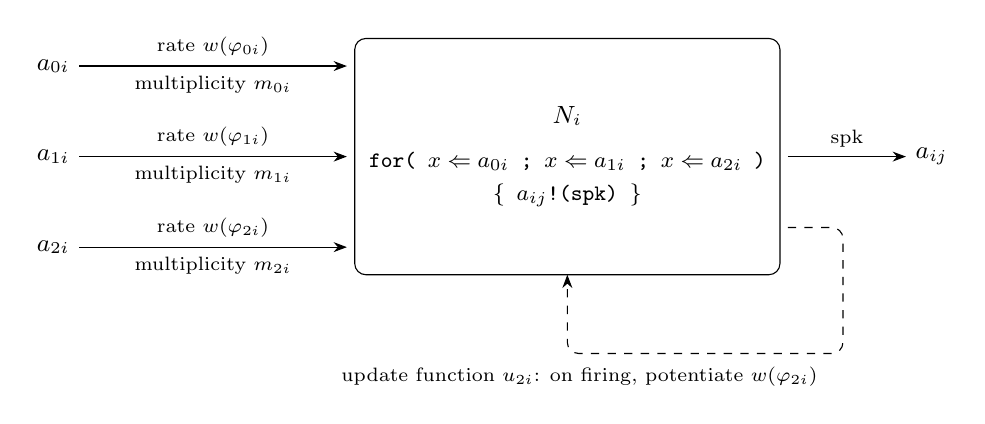
\begin{tikzpicture}[>=Stealth]
  \node[draw, rounded corners, minimum width=54mm, minimum height=30mm, align=center] (N) at (0,0)
    {\small $N_i$\\[4pt]
     \footnotesize\ttfamily for( $x\Leftarrow a_{0i}$ ; $x\Leftarrow a_{1i}$ ; $x\Leftarrow a_{2i}$ )\\
     \footnotesize\ttfamily \{\ $a_{ij}$!(spk)\ \}};
  \foreach \k/\y in {0/1.15, 1/0.0, 2/-1.15} {
    \node[anchor=east] (d\k) at (-6.2,\y) {\small $a_{\k i}$};
    \draw[->] (d\k.east) -- node[above, font=\scriptsize, pos=0.5] {rate $\wmap(\varphi_{\k i})$}
              node[below, font=\scriptsize, pos=0.5] {multiplicity $m_{\k i}$} (-2.8,\y);
  }
  \node[anchor=west] (o) at (4.3,0) {\small $a_{ij}$};
  \draw[->] (2.8,0) -- node[above, font=\scriptsize] {spk} (o.west);
  \draw[->, dashed, rounded corners]
    (2.8,-0.9) -- (3.5,-0.9) -- (3.5,-2.5) -- (0,-2.5) -- (0,-1.5);
  \node[font=\scriptsize, anchor=north east] at (3.3,-2.55)
    {update function $u_{2i}$: on firing, potentiate $\wmap(\varphi_{2i})$};
\end{tikzpicture}
\caption{A neuron. The three factors of Definition~\ref{def:propensity} are visible: the weight map
supplies a rate constant per synapse, the marking supplies multiplicity, and the geometric factor is
$1$. The dashed arrow is the refinement entry's update function, which is where plasticity lives.}
\label{fig:neuron}
\end{figure}

\subsection{The keys, and why they form a partition}

\begin{definition}[Synaptic keys]
\label{def:synkeys}
For each synapse $(j,i)$ put
\[
\varphi_{ji} \;\;\triangleq\;\; \inn(a_{ji})\top \;\sepc\; \out(a_{ji})\top ,
\]
the formula holding of a communication redex on $a_{ji}$, and let
$\Phi_{\textsc{comm}} = \{\varphi_{ji}\} \cup \{\varphi_\bot\}$ with
$\varphi_\bot = L^\sharp \wedge \neg\bigvee_{ji}\varphi_{ji}$.
\end{definition}

\begin{proposition}
\label{prop:rnn-admissible}
$\Phi_{\textsc{comm}}$ is admissible, with $\alpha = 2$.
\end{proposition}

\begin{proof}
Distinct synapses are distinct channels, and a communication redex is on exactly one channel, so
(P1) holds; $\varphi_\bot$ gives (P2) by Remark~\ref{rem:default}. Each key has depth $2$ by
Definition~\ref{def:depth}, and checking $\inn(a)\top \sepc \out(a)\top$ against a term is a bag
lookup, so \ref{req:dec} and \ref{req:loc} hold.
\end{proof}

The weight $\wmap(\varphi_{ji})$ is the efficacy of synapse $(j,i)$. Nothing else in the presentation
mentions it.

\subsection{Threshold is join structure}

\begin{proposition}[McCulloch--Pitts]
\label{prop:mcp}
The threshold presentation of Definition~\ref{def:neuron} realises the monotone Boolean threshold
function $\mathbf{1}[\,\sum_{j} \mathbf{1}[a_{ji}\text{ populated}] \geq \theta_i\,]$: the neuron has
an enabled redex exactly when at least $\theta_i$ of its dendrites carry a pending spike. It uses
$\binom{k_i}{\theta_i}$ join groups.
\end{proposition}

\begin{proof}
A group $S$ is enabled iff every $a_{si}$ for $s \in S$ carries a spike, since $\&$ requires
simultaneous availability of all its binds; the receipt is enabled iff some group is, since $;$
separates alternatives. Some $\theta_i$-subset is fully populated iff at least $\theta_i$ dendrites
are populated. The count of groups is the count of $\theta_i$-subsets.
\end{proof}

So the historical origin of the neuron model --- McCulloch and Pitts' threshold unit \cite{mcp} ---
is not encoded in a weighted GSLT but \emph{is} a for-comprehension, with the threshold appearing as
the arity of the joins and the alternatives as the group separator. Two remarks temper this.

\begin{remark}[The combinatorial blowup, and the \texttt{where} clause]
$\binom{k}{\theta}$ groups is unusable for realistic fan-in. Rholang~1.4's for-comprehension carries
a \texttt{where} clause \cite{omnibus}, which collapses the presentation to a single group at the
cost of changing the semantics: \texttt{for($x_1 \Leftarrow a_{1i}\ \&\ \cdots\ \&\ x_k \Leftarrow
a_{ki}$ where $\phi$)} waits for \emph{all} $k$ dendrites and then gates on $\phi$. That is a
coincidence detector with a filter, not a threshold unit. The two presentations agree at
$\theta = k$ and differ elsewhere, and which one a modeller wants is a modelling question. We use
$\theta_i = 1$ below, where both are trivial and the group presentation has $k_i$ single-bind
alternatives.
\end{remark}

\begin{remark}[Coincidence versus rate]
$\theta_i = k_i$ gives a pure coincidence detector: the neuron fires only on simultaneous arrival at
every dendrite. $\theta_i = 1$ gives a pure rate integrator: any arrival can trigger it, and the
weights determine how fast. Real cortical neurons sit between, and so does the presentation, with
$\theta$ as the dial. This is a rare case in which a biological parameter and a syntactic parameter
are the same parameter.
\end{remark}

\subsection{The weighted sum, and where the squashing function went}
\label{sec:squash}

Take $\theta_i = 1$, so $N_i$ has $k_i$ single-bind alternatives, and let the marking assign $m_{ji}$
pending spikes to dendrite $a_{ji}$.

\begin{proposition}[Propensity of a neuron]
\label{prop:neuron-prop}
With $\gfac \equiv 1$ and $\chi \equiv 1$, the total propensity of the redexes belonging to neuron
$i$ is
\[
\prop_i \;=\; \sum_{j} \wmap(\varphi_{ji}) \cdot m_{ji} .
\]
\end{proposition}

\begin{proof}
The receipt is persistent, so exactly one input is available on each $a_{ji}$, and the marking
supplies $m_{ji}$ outputs; by Definition~\ref{def:redex} the number of redexes classified $\varphi_{ji}$
is $1 \cdot m_{ji}$. Definition~\ref{def:propensity} gives $\wmap(\varphi_{ji})m_{ji}$ per synapse,
and the classes are disjoint by Proposition~\ref{prop:rnn-admissible}, so
Proposition~\ref{prop:total} lets them be summed.
\end{proof}

This is exactly the weighted sum $\sum_j w_{ji} m_{ji}$ of the textbook artificial neuron, with the
presynaptic activity $m_{ji}$ read as the marking. It has not been written into any term; it is the
propensity that Definition~\ref{def:propensity} computes.

\begin{corollary}[The response is logistic and nobody wrote it]
\label{cor:sigmoid}
Hold the marking fixed over a short window $[0,\Delta]$. The probability that neuron $i$ fires at
least once in the window is
\[
\Pr[\,\text{$i$ fires}\,] \;=\; 1 - \exp\!\big(-\Delta \textstyle\sum_j \wmap(\varphi_{ji}) m_{ji}\big),
\]
a saturating, monotone function of the weighted sum, with slope $\Delta$ at the origin and asymptote
$1$.
\end{corollary}

\begin{proof}
Firings of $i$ within the window are the events of a Poisson process of rate $\prop_i$ under the
frozen marking, by Theorem~\ref{thm:markov} restricted to the sub-chain in which no other transition
alters $m_{\cdot i}$.
\end{proof}

The proviso is real: the marking is not in fact frozen, since other neurons are firing into it, and
Corollary~\ref{cor:sigmoid} is a statement about a window short enough that the input has not moved.
That is the usual justification for a rate-coded neuron, and it is the usual approximation. What is
not an approximation is the observation that no squashing function was supplied. The saturation is
the exponential waiting-time law of the chain: a neuron with enormous drive cannot fire more than
once per event, so its firing probability per window is bounded by $1$ no matter how large the sum
gets. The logistic nonlinearity of the artificial neuron is a compressed description of a Poisson
process, and here it is the Poisson process.

\subsection{Boundedness}

\begin{lemma}[Boundedness]
\label{lem:bounded}
Let $f_i = |\mathrm{post}(i)|$ be the fan-out of neuron $i$. If $f_i \leq \theta_i$ for every $i$,
the total number of pending spikes is non-increasing along every run, the reachable term set is
finite, and $\mathsf{Net}$ is term-finite in the sense of Definition~\ref{def:bounded}.
\end{lemma}

\begin{proof}
Firing $N_i$ consumes $\theta_i$ pending spikes (one per bind in the selected group) and produces
$f_i$. The total marking therefore changes by $f_i - \theta_i \leq 0$. Since the neurons are
persistent and the channel set is fixed, a term reachable from $\mathsf{Net}$ is determined by its
marking, and markings with at most $|M_0|$ tokens over finitely many channels are finite in number.
\end{proof}

The hypothesis is restrictive: it forbids fan-out exceeding threshold, which most networks want. Two
standard repairs, both expressible in the theory:

\begin{enumerate}[leftmargin=2.2em]
\item \emph{Capacity.} Guard the neuron body's sends by a \texttt{where} clause bounding the
occupancy of the target channel by $c$. The marking is then bounded by $c$ per channel and the state
space by $c^{|\vec a|}$, restoring term-finiteness unconditionally. This is a saturating synapse, and
it is what a real one does.
\item \emph{Leak.} Add a base rule $a_{ji}!(\mathrm{spk}) \leadsto \Nil$ with its own key and weight
$\lambda_{\text{leak}}$. This does not restore term-finiteness by itself but makes the marking
positive-recurrent, which is enough for the stationary analysis and for classical simulation, though
not for \S\ref{sec:quantum}.
\end{enumerate}

We take capacity in what follows, since \S\ref{sec:rnn-quantum} needs a finite-dimensional
$\mathcal{H}$.

\begin{remark}[The network is a marked graph]
Under Lemma~\ref{lem:bounded}, $\mathsf{Net}$ is a live, bounded, conservative marked graph in the
Petri-net sense, and the analysis of \cite{knots} applies verbatim: a \emph{period} is a firing
schedule returning the marking to its initial value, and it is the right analogue of a timestep. The
weighted-GSLT layer adds what a marked graph does not have, namely a probability distribution over
which of the enabled transitions fires next and how long it takes.
\end{remark}

\subsection{Plasticity is the update function}
\label{sec:plasticity}

\begin{definition}[Hebbian entry]
\label{def:hebb}
Equip the communication rule's entry at $\varphi_{ji}$ with
\[
u_{ji}(\wmap) \;=\; \wmap\big[\,\varphi_{ji} \mapsto \min\{\,w_{\max},\ \wmap(\varphi_{ji}) + \eta\,\}\,\big],
\]
for a potentiation increment $\eta > 0$ and ceiling $w_{\max}$.
\end{definition}

So the augmented rule reads, in full:
\begin{center}
\begin{minipage}{0.92\textwidth}
\begin{lstlisting}
COMM . |- (PPar {(PForUser rows p), (POutput n q), ...rest})
        ~> (PPar {(subst ...), ...rest})  [1.0] {
      phi(0,1) => (w_01, hebb(0,1)),
      phi(1,1) => (w_11, hebb(1,1)),
      ...
      phi_bot  => (0.0,  id)
   };
ParCong . | S ~> T |- (PPar {S, ...rest}) ~> (PPar {T, ...rest})  [1.0] { snd };
\end{lstlisting}
\end{minipage}
\end{center}

\begin{theorem}[Learning and inference are one relation]
\label{thm:one-relation}
Let $\mathsf{Net}$ be a weighted GSLT as above. The transition relation of
Definition~\ref{def:transition} on $\Cfg = \Terms \times \Wt$ has two marginals: the projection to
$\Terms$ is the network's inference dynamics, and the projection to $\Wt$ is its learning dynamics.
Neither is a separate process. In particular there is no training schedule, no separate learning
clock, and no distinguished learning phase; the learning rate $\eta$ is not a hyperparameter of an
outer loop but a component of the theory, sitting in the same refinement entry as the weight it
modifies.
\end{theorem}

\begin{proof}
Immediate from Definitions~\ref{def:config} and \ref{def:transition}: a single step produces
$(P', \wmap')$ with $P'$ obtained by the rewrite and $\wmap'$ by the fold of the update function.
\end{proof}

This is the claim the example exists to make, and it is exactly what a static-rate calculus cannot
express. In SPiM a rate is fixed at declaration, so a stochastic $\pi$ model of a neural network can
model the firing but not the learning; one must step outside the calculus, adjust the rates, and
re-run. Here the adjustment is a transition of the same system.

\begin{remark}[Cells that fire together wire together, literally]
Definition~\ref{def:hebb} potentiates $\varphi_{ji}$ when a communication on $a_{ji}$ fires --- that
is, when a presynaptic spike is consumed by a postsynaptic receipt. The condition ``pre and post were
jointly involved in an event'' is not a correlation computed by an observer; it is the firing of a
single rewrite, which by construction requires both parties. Hebb's rule is the statement that the
event which transmits is the event which potentiates \cite{hebb}, and here those are the same event
because a communication is one rewrite.
\end{remark}

\subsection{Spike-timing dependence needs a wider update signature}
\label{sec:stdp}

Spike-timing-dependent plasticity makes $\Delta w$ a function of the interval between pre- and
postsynaptic spikes, potentiating for pre-before-post and depressing for the reverse \cite{stdp}.
The ingredients are available --- the simulator of Definition~\ref{def:ssa} produces a timestamp at
every step --- but the update function of Definition~\ref{def:augmented} cannot see them, since its
type is $\Wt \to \Wt$.

\begin{definition}[Extended update]
\label{def:extended-update}
Replace $u_i : \Wt \to \Wt$ by
\[
u_i \;:\; \Wt \times \mathrm{Match} \times \partial\Terms \times \mathbb{R}_{\geq 0} \times \mathcal{S} \longrightarrow \Wt ,
\]
taking additionally the matched substitution $\sigma$, the position $k$ at which the rule fired, the
current simulation time $t$, and a bounded \emph{trace summary} $\mathcal{S}$ --- for STDP, one
eligibility trace per synapse, itself decaying at a rate specified in the theory.
\end{definition}

Theorem~\ref{thm:markov} survives this extension provided $\mathcal{S}$ is finite-dimensional and
updated deterministically, since one simply enlarges the configuration to
$(P, \wmap, \mathcal{S})$; it does \emph{not} survive an update function reading unbounded history,
which would make the process genuinely non-Markovian and put exact simulation out of reach. The
eligibility-trace formulation of STDP is precisely the standard device for staying inside the
bounded case, and it is pleasant that the constraint arrives here from the requirement that the
chain be a chain rather than from computational convenience.

\subsection{Uniformity: one theory for every network}
\label{sec:rnn-uniform}

Definition~\ref{def:synkeys} gives one key per synapse, so a network with $10^4$ synapses has $10^4$
keys and a network that grows needs a new theory. Reflection removes both problems. Following the
construction of \cite{knots}, take the synapse channels to be structured names
\[
a_{ji} \;=\; @[\,*\mathit{net},\, j,\, i\,],
\]
so that a name predicate can recover the endpoints. Then
\[
\varphi_{\mathrm{syn}} \;\triangleq\; \exists j, i.\; \inn(@[*\mathit{net},j,i])\top \;\sepc\; \out(@[*\mathit{net},j,i])\top
\]
is a single key describing the whole \emph{namespace} of synapses of this network, which is
namespace logic doing what it was built for \cite{namespace}. The weight map then has one entry per
network rather than per synapse; per-synapse efficacies are recovered by letting the entry's value be
a function of the recovered indices, which is the standard move of trading a large map for a small
map with structured keys. A greatest fixed point makes ``every neuron reachable from $i$ eventually
fires'' a single formula rather than an $n$-fold conjunction, which is the uniformity $\nu$ buys
\cite[\S3]{classifier}. In an atomic-name calculus none of this is available: the indices would have
to travel as message payloads and the logic could reach them only by observing traffic.

\subsection{The quantum network}
\label{sec:rnn-quantum}

Replace the efficacies by amplitudes $z_{ji} \in \Cx$, $|z_{ji}| \leq 1$, keeping the keys, the
neurons, and the capacity bound. Definition~\ref{def:jump} gives a jump operator per synapse,
Definition~\ref{def:qctmc} a Lindbladian, and Definition~\ref{def:qjump} a trajectory simulator.
Because the capacity bound makes $\mathcal{B}$ finite, $\mathcal{H}$ is finite-dimensional and the
model checking of \cite{qctmc,qctmc-csl} applies, with the projectors supplied by
Proposition~\ref{prop:projective} --- for instance $\Pi_{\varphi_{\mathrm{syn}}}$, whose expectation
is the probability that the network has an available synaptic transmission at time $t$.

\begin{remark}[Indistinguishable spikes interfere]
\label{rem:bosonic}
By Remark~\ref{rem:distinct-contracta}, $m$ indistinguishable pending spikes on $a_{ji}$ give $m$
redexes with a common contractum. Classically their rates add and the transition runs at
$m \cdot \wmap(\varphi_{ji})$. In the complex case their \emph{amplitudes} add, so the amplitude to
the target is $m\,z_{ji}$ and the probability weight is $m^2 |z_{ji}|^2$. The quantum network is
therefore not the classical one with phases attached: it is superlinear in presynaptic multiplicity
where the classical one is linear, and the enhancement is exactly a consequence of the spikes being
elements of a bag rather than a list. Whether that is a feature or an artefact of the encoding is a
genuine question --- one could break the degeneracy by tagging spikes, recovering linearity --- and
we flag it rather than settle it.
\end{remark}

\subsection{What this example does not show}

Honesty about scope. The learning here is local and Hebbian; nothing above implements
backpropagation, which needs a global error signal propagated against the direction of inference.
One can encode such a signal as traffic on a second family of channels with its own keys, and the
apparatus does not forbid it, but the result would no longer have the property that makes
Theorem~\ref{thm:one-relation} interesting --- the error channel is an outer loop wearing a costume.
Whether a genuinely local weighted-GSLT learning rule can match backpropagation is not a question
this note answers, and the honest statement is that the example demonstrates a \emph{mechanism} for
plasticity inside the calculus, not a competitive learning algorithm.

Nor do we claim biological fidelity. The neuron of Definition~\ref{def:neuron} has no membrane
potential, no refractory period, and no dendritic geometry. The first two are easy additions --- a
potential is a payload, a refractory period is a guard --- and the third is what the geometric factor
$\gfac$ of \S\ref{sec:geometric} is for, which is a use we have not developed.

\section{Implementation}
\label{sec:impl}

\subsection{Surface syntax}

The weighting is a decoration of MeTTaIL's \texttt{rewrites} block, and it should read as one. The
existing surface is
\begin{center}
\begin{minipage}{0.88\textwidth}
\begin{lstlisting}
rewrites {
    Exec    . |- (PDrop (NQuote P)) ~> P;
    ParCong . | S ~> T |- (PPar {S, ...rest}) ~> (PPar {T, ...rest});
}
\end{lstlisting}
\end{minipage}
\end{center}
and the weighted surface adds a bracketed weight and a brace block after the rule, in both cases
optional:
\begin{center}
\begin{minipage}{0.88\textwidth}
\begin{lstlisting}
rewrites {
    // base rule: [scalar] { key => (weight, update) }
    COMM . |- (PPar {(PForUser rows p), (POutput n q), ...rest})
            ~> (PPar {(subst rows p q), ...rest})   [1.0] {
        in(n)TOP | out(n)@fast  => (2.5, scale(0.9)),
        in(n)TOP | out(n)TOP    => (0.7, id),
        default                 => (0.0, id)
    };

    // base rule, unweighted: defaults to [1.0] { default => (1.0, id) }
    Exec . |- (PDrop (NQuote P)) ~> P;

    // context rule: [geometric factor] { fold }
    ParCong . | S ~> T |- (PPar {S, ...rest}) ~> (PPar {T, ...rest})  [1.0] { snd };
}
\end{lstlisting}
\end{minipage}
\end{center}

Notes on the design. \texttt{default} is sugar for the completion of
Remark~\ref{rem:default} --- the elaborator synthesises
$L^\sharp \wedge \neg\bigvee_i \varphi_i$ --- so a modeller writes exclusive keys and gets a
partition. Exclusivity itself is checked at elaboration time and is a hard error, not a warning,
since Proposition~\ref{prop:classify} fails without it. Keys are written in the concrete syntax of
the generated logic; the two shown are ordered from more to less specific purely for readability,
since exclusivity means order is semantically irrelevant. A context rule's default factor is
$1$ and its default fold is \texttt{snd}, which together implement ``addressing is free and does not
touch the map'' (\S\ref{sec:geometric}).

\subsection{Delta against the prototype}

The prototype at \texttt{rho-life/Gillespie} \cite{gillespie-crate} implements a substantial part of
this. The following is what separates it from the specification above, in descending order of
importance.

\begin{enumerate}[leftmargin=2.2em]
\item \emph{Propensity ignores the term.} \texttt{BaseRule::propensity()} returns the rule weight
times the sum of its refinement weights, with no dependence on the configuration. Gillespie's multiplicity factor --- the cardinality of $K(r,\varphi,P)$ in
Definition~\ref{def:propensity} --- is absent, so a term with fifty available redexes of a kind fires
them no faster than a term with one. This is the one correctness bug rather than a design
divergence, and it requires a matcher over the term, which the crate does not currently have (its
\texttt{TermRef} is an opaque id, sort and display string).
\item \emph{Spatial behaviours are hand-rolled.} The \texttt{SpatialBehavior} enum
(\texttt{Local}, \texttt{Interaction}, \texttt{Parallel}, \texttt{Sequential}, \texttt{Guard},
\texttt{Replicated}, \texttt{Custom}) is a fixed vocabulary written by hand. Keys must instead be
formulae of the logic \emph{generated} from the language spec, or the construction loses the property
that makes it generic over GSLTs. This is the largest gap between crate and specification and the
one gated on the branch's logic work.
\item \emph{No partition check.} Nothing enforces (P1) or (P2), and \texttt{RateMap::select\_classical}
picks by cumulative weight over the entries as declared, which silently implements the
``sum over all satisfied keys'' aggregation. Elaboration-time exclusivity checking and
\texttt{default} synthesis are required.
\item \emph{Context rules carry independent propensity.} \texttt{ContextRule} has its own weight and
enters the propensity sum alongside base rules, which double-counts (\S\ref{sec:geometric}). It
should contribute $\gfac(k)$ multiplicatively to the base firing it addresses.
\item \emph{Rates are clamped to $[0,1]$.} \texttt{RateValue::real} rejects values outside the unit
interval and \texttt{RateValue::add} clamps sums to $1$. Per Remark~\ref{rem:rnn} the codomain is
$\Rnn$; the clamping additionally makes $\prop_0$ wrong whenever two classes are simultaneously
enabled with rates summing above $1$.
\item \emph{Update functions are too narrow.} \texttt{UpdateFn = Fn(\&RateMap) -> RateMap} cannot see
the match, the position, or the clock, so Definition~\ref{def:hebb} is expressible but
\S\ref{sec:stdp} is not. Widen to Definition~\ref{def:extended-update}.
\item \emph{The quantum module is not a QCTMC.} \texttt{quantum.rs} maintains a
superposition of \texttt{(TermRef,}\allowbreak\ \texttt{Complex64,}\allowbreak\ \texttt{RateMap)}
triples and measures by $|z|^2$. That is amplitude
bookkeeping over a classical branching structure; reaching \cite{qctmc} needs density operators, the
jump operators of Definition~\ref{def:jump}, the Lindbladian of Definition~\ref{def:qctmc}, and the
non-Hermitian evolution of Definition~\ref{def:qjump}. In particular there is currently no $\Heff$,
so the waiting time cannot be drawn from a decaying norm and
Theorem~\ref{thm:jump-gillespie}'s general case is unreachable.
\item \emph{Syntax drift.} \texttt{language\_ext.rs} documents context rules as
\texttt{if <cond> then <lhs> \textasciitilde> <rhs>}, where MeTTaIL writes
\texttt{| S \textasciitilde> T |- \dots}. Also, \texttt{lib.rs} declares a \texttt{fuzzer} module
that is not present in the tree.
\end{enumerate}

Items 1, 3, 4, 5 and 8 are local and can be done now. Item 6 is a signature change with a
configuration-space consequence (\S\ref{sec:stdp}). Item 2 is gated on the generated logic, which is
still under development in the feature branch; until it lands, the honest interim is to keep a
hand-rolled key vocabulary but to make it an \emph{adapter} behind the same interface the generated
formulae will implement, so the swap is at the boundary rather than through the simulator. Item 7 is
a rewrite of one module.

\subsection{Incremental propensity}

Lemma~\ref{lem:locality} licenses the standard optimisation. Maintain $\prop$ as a Fenwick tree over
$(r,\varphi)$ classes with per-class redex lists; after firing at position $k$, reclassify only
redexes within radius $\alpha + |L| + |R|$ of $k$, and additionally rescale the classes whose weight
the update function touched --- which for Definition~\ref{def:hebb} is exactly one class. The second
part is the only respect in which dynamic weight maps cost anything at run time, and it is cheap
precisely when update functions are sparse. A modeller who writes an update function touching every
entry pays a full recomputation of $\prop_0$ per step, and should be told so.

\section{Weights and costs}
\label{sec:cost}

Cost accounting and weighting both decorate rewrites, and it is worth stating plainly that they are
different decorations doing different jobs.

A cost decoration attaches to a rewrite a debit against a token stack, and the funding judgment
$\Sigma \funds \Delta$ --- decidable, total, monotone in supply --- decides whether a step may occur
at all \cite{costmonad}. It is implemented in the transpiler branch as
\texttt{OslfResourceLogic}, with a supply multiset keyed by signature and a demand list, one token
per signed term, and conformance laws asserting soundness, rejection of underfunding, supply
monotonicity, and decidability. A weight decoration attaches a rate, and decides how fast and how
often. The composition is one-directional:

\begin{definition}[Funding gate]
\label{def:gate}
For a redex $(k,\sigma)$ of rule $r$, let $\Delta(r,k,\sigma)$ be the demand it incurs and
$\Sigma(P,k)$ the supply available at that location. Put
$\chi(r,k,\sigma) = 1$ if $\Sigma(P,k) \funds \Delta(r,k,\sigma)$ and $0$ otherwise.
\end{definition}

\begin{proposition}[Cost gates the support, weight distributes over it]
\label{prop:gate}
With $\chi$ as in Definition~\ref{def:gate}, the coalgebra of Definition~\ref{def:coalgebra}
restricts to the funded sub-transition-system: unfunded redexes have propensity zero and contribute
nothing to $\prop_0$, while among funded redexes the distribution is unchanged from the
cost-free case up to normalisation.
\end{proposition}

\begin{proof}
$\chi$ appears as a multiplicative factor in Definition~\ref{def:propensity}, taking values in
$\{0,1\}$; a zero factor removes the term from the sum, and the remaining terms are untouched.
\end{proof}

Three consequences worth recording.

\emph{The gate is decidable, so the simulator stays exact.} If funding were a real-valued penalty
rather than a Boolean, the propensity would depend on an optimisation and the chain would no longer
be simulable by Definition~\ref{def:ssa}. The decidability law of the resource logic is doing real
work here.

\emph{Exhaustion is a halting condition, not a deadlock.} $\prop_0 = 0$ when every enabled redex is
unfunded, and Definition~\ref{def:ssa} halts. The chain has reached an absorbing state, which is the
correct reading: a system that cannot pay for any of its available transitions has stopped, and the
waiting time to the next event is infinite rather than undefined.

\emph{The neural example acquires a metabolism.} Give the communication rule a phlogiston demand per
firing and the network of \S\ref{sec:rnn} has an energy budget: a neuron whose local supply is
exhausted has propensity zero regardless of its synaptic weights, and the network's activity is
bounded by its funding rather than by its capacity guard. Weight is what a synapse is worth; cost is
what a spike costs. Separating them is what lets a model say that a strong synapse on a starving
neuron is silent, which is a statement neither decoration makes alone. This is the point of contact
with the mortal-computation reading of \cite{scientist}, and we go no further with it here.

\section{Open threads}
\label{sec:open}

\begin{enumerate}[leftmargin=2.2em]
\item \emph{A combined logic.} \S\ref{sec:qctmc-logic} has the generated logic supplying projectors
to an external temporal logic. What one wants is a single logic with context-labelled modalities and
time-bounded operators --- $\langle K_j \rangle^{\leq t}\varphi$ --- adequate for weighted
bisimulation on configurations. The classical half of this is well trodden (CSL over CTMCs); the
question is what OSLF emits when the presentation it is fed is already weighted.
\item \emph{Weighted bisimulation.} The category \textbf{GSLT} has bisimulation-preserving maps as
morphisms \cite{omnibus}. What is the right notion when the objects carry weight maps? Rate
bisimulation (lumpability) is the obvious candidate for $\Rnn$; the $\Cx$ case has no obvious
candidate, and the interference of Proposition~\ref{prop:interference} suggests it should not be a
relation on terms alone.
\item \emph{Geometric factors.} \S\ref{sec:geometric} identifies $\gfac$ as the natural home of a
spatial weighting and declines to develop it. The gravitation correspondence of
\cite{costspacetime} splits a weight on a reduction-graph edge into a geometric part and a matter
part; here $\gfac(k)$ is visibly the first and $\wmap(\varphi)$ visibly the second, and the
correspondence asks for an action forcing the two to agree. That is a paper.
\item \emph{Quantale weights.} A quantale-valued codomain gives a fuzzy calculus, and \cite{fuzzy}
develops the flat-substitution instance independently. Whether it is an instance of
Definition~\ref{def:wmap} or a genuinely different decoration --- the fuzzy comm rule transmits a
modified payload, which no weighting here does --- is not settled, and settling it is the natural
way to test whether $\mathcal{K}$ is really a parameter.
\item \emph{Map-finiteness.} \S\ref{sec:finiteness} notes that plastic weights leave the reachable
map set infinite unless quantised or saturated. Quantised weights make $\Cfg$ finite and the whole
apparatus model-checkable; they also make the learning dynamics a finite automaton, whose reachable
weight configurations are an object nobody has looked at.
\item \emph{The bosonic enhancement.} Remark~\ref{rem:bosonic} observes that indistinguishable
messages give amplitude $m z$ rather than rate $m|z|^2$, so the quantum reading is superlinear in
multiplicity. Whether this is a feature of the physics being modelled or an artefact of the
associative--commutative presentation is open, and it is the sharpest available test of whether the
complex case is a genuine quantum semantics or a formal analogy.
\end{enumerate}

\begin{thebibliography}{99}

\bibitem{classifier} L.\ G.\ Meredith. \emph{Classifying knots with spatial--behavioural logics.}
F1R3FLY.io working note, 2026.

\bibitem{costmonad} L.\ G.\ Meredith. \emph{Cost accounting as an endofunctor on continued
interactive GSLTs.} F1R3FLY.io working note, 2026.

\bibitem{costspacetime} L.\ G.\ Meredith. \emph{Cost, spacetime, and the geometry/matter split on
reduction graphs.} F1R3FLY.io working notes, 2026.

\bibitem{dalibard} J.\ Dalibard, Y.\ Castin and K.\ M\o lmer. Wave-function approach to dissipative
processes in quantum optics. \emph{Physical Review Letters} 68(5):580--583, 1992.

\bibitem{fuzzy} \emph{Fuzzy rho-calculus: a quantale-graded interaction, and its lift to ciGSLTs with
binding.} F1R3FLY.io working note, 2026.

\bibitem{gibson-bruck} M.\ A.\ Gibson and J.\ Bruck. Efficient exact stochastic simulation of
chemical systems with many species and many channels. \emph{Journal of Physical Chemistry A}
104(9):1876--1889, 2000.

\bibitem{gillespie77} D.\ T.\ Gillespie. Exact stochastic simulation of coupled chemical reactions.
\emph{Journal of Physical Chemistry} 81(25):2340--2361, 1977.

\bibitem{gillespie-crate} F1R3FLY.io. \texttt{mettail-gillespie}: stochastic and quantum Gillespie
simulation extensions for MeTTaIL rewrite rules. \texttt{F1R3FLY-io/publications},
\texttt{rho-life/Gillespie}, 2026.

\bibitem{hebb} D.\ O.\ Hebb. \emph{The Organization of Behavior.} Wiley, 1949.

\bibitem{knots} L.\ G.\ Meredith. \emph{Knots as cost-accounted processes.} F1R3FLY.io working note,
2026.

\bibitem{mcp} W.\ S.\ McCulloch and W.\ Pitts. A logical calculus of the ideas immanent in nervous
activity. \emph{Bulletin of Mathematical Biophysics} 5:115--133, 1943.

\bibitem{mcwf} K.\ M\o lmer, Y.\ Castin and J.\ Dalibard. Monte Carlo wave-function method in quantum
optics. \emph{Journal of the Optical Society of America B} 10(3):524--538, 1993.

\bibitem{mettacalc} L.\ G.\ Meredith et al. \emph{The MeTTa calculus.} F1R3FLY.io, 2026.

\bibitem{mettail} F1R3FLY.io. \texttt{mettail-rust}: the \texttt{language!} macro and its shipped
language definitions. \texttt{F1R3FLY-io/mettail-rust}, 2026.

\bibitem{namespace} L.\ G.\ Meredith and M.\ Radestock. Namespace logic: a logic for a reflective
higher-order calculus. In \emph{Trustworthy Global Computing}, LNCS 3705, Springer, 2005.

\bibitem{omnibus} L.\ G.\ Meredith. \emph{Graph-Structured Lambda Theories: A Reference for the
Working Developer.} F1R3FLY.io, 2026.

\bibitem{priami} C.\ Priami. Stochastic $\pi$-calculus. \emph{The Computer Journal} 38(7):578--589,
1995.

\bibitem{scientist} L.\ G.\ Meredith. \emph{The Mortal Scientist.} F1R3FLY.io working note, 2026.

\bibitem{spim} A.\ Phillips and L.\ Cardelli. A correct abstract machine for the stochastic
pi-calculus. In \emph{Bioconcur}, 2004.

\bibitem{spim-sim} A.\ Phillips and L.\ Cardelli. Efficient, correct simulation of biological
processes in the stochastic pi-calculus. In \emph{Computational Methods in Systems Biology}, LNCS
4695, Springer, 2007.

\bibitem{stdp} G.\ Q.\ Bi and M.\ M.\ Poo. Synaptic modifications in cultured hippocampal neurons:
dependence on spike timing, synaptic strength, and postsynaptic cell type. \emph{Journal of
Neuroscience} 18(24):10464--10472, 1998.

\bibitem{qctmc} M.\ Xu, J.\ Mei, J.\ Guan and N.\ Yu. Model checking quantum continuous-time Markov
chains. In \emph{CONCUR 2021}, LIPIcs 203, 13:1--13:17. Schloss Dagstuhl, 2021. Preprint
\texttt{arXiv:2105.00382}.

\bibitem{qctmc-csl} M.\ Xu, J.\ Mei, J.\ Guan and N.\ Yu. Checking continuous stochastic logic
against quantum continuous-time Markov chains. \emph{Logical Methods in Computer Science}, 2025.
Preprint \texttt{arXiv:2202.05412}.

\end{thebibliography}

\end{document}
